%%%%%%%%%%%%%%%%%%%%%%%%%%%%%%%%%%%%%%%%%%%%%%%%%%%%%%%%%%%%%%%%%%%%%%%%%%%%%%%%%%%
%% This project aims to create the UFC template for presentation.                %%
%% author: Maurício Moreira Neto - Doctoral student in Computer Science (MDCC)   %%
%% contacts:                                                                     %%
%%    e-mail: maumneto@ufc.br                                                    %%
%%    linktree: https://linktr.ee/maumneto                                       %%
%%%%%%%%%%%%%%%%%%%%%%%%%%%%%%%%%%%%%%%%%%%%%%%%%%%%%%%%%%%%%%%%%%%%%%%%%%%%%%%%%%%
\documentclass{libs/ufc_format}
% Inserting the preamble file with the packages
%%%%%%%%%%%%%%%%%%%%%%%%%%%%%%%%%%%%%%%%%%%%%%%%%%%%%%%%%%%%%%%%%%%%%
%% This file contains the packages that can be used in the beamer. %%
%%%%%%%%%%%%%%%%%%%%%%%%%%%%%%%%%%%%%%%%%%%%%%%%%%%%%%%%%%%%%%%%%%%%%
% Package to fonts family
\usepackage[T1]{fontenc}
% Package to accentuation
\usepackage[utf8]{inputenc}
% Package to Portuguese language
\usepackage[brazil]{babel}
% Package to Figures
\usepackage{graphicx}
% Package to the colors
\usepackage{color}
% Package to the colors
\usepackage{xcolor}
% Packages to math symbols and expressions
\usepackage{amsfonts, amssymb, amsmath}
% Package to multiple lines and columns in table
\usepackage{multirow, array} 
% Package to create pseudo-code
% For more detail of this package: http://linorg.usp.br/CTAN/macros/latex/contrib/algorithm2e/doc/algorithm2e.pdf
\usepackage{algorithm2e}
% Package to insert code
\usepackage{listings} 
\usepackage{keyval}
% Package to justify text
\usepackage[document]{ragged2e}
% Package to manage the bibliography
\usepackage[backend=biber, style=numeric, sorting=none]{biblatex}
% Package to facilities quotations
\usepackage{csquotes}
% Package to use multicols
\usepackage{multicol}


%% On my own
\newcommand{\aspas}[1]{``#1''}

% Inserting the references file
\bibliography{references.bib}

% Title
\title[Aprendizado Estatístico em Dados Longitudinais]{\huge\textbf{Aprendizado Estatístico em Dados Longitudinais}}
% Subtitle
\subtitle{}
% Author of the presentation
\author{Cícero Hitzschky}
% Institute's Name
\institute[UFC]{
    % email for contact
    \normalsize{\email{cicero.hitzschky@alu.ufc.br}}
    \newline
    % Department Name
    \department{Departamento de Estatística e Matemática Aplicada}
    \newline
    % university name
    \ufc
}
% date of the presentation
\date{\today}


%%%%%%%%%%%%%%%%%%%%%%%%%%%%%%%%%%%%%%%%%%%%%%%%%%%%%%%%%%%%%%%%%%%%%%%%%%%%%%%%%%
%% Start Document of the Presentation                                           %%               
%%%%%%%%%%%%%%%%%%%%%%%%%%%%%%%%%%%%%%%%%%%%%%%%%%%%%%%%%%%%%%%%%%%%%%%%%%%%%%%%%%
\begin{document}
% insert the code style
%%%%%%%%%%%%%%%%%%%%%%%%%%%%%%%%%%%%%%%%%%%%%%%%%%%%%%%%%%%%%%%%%%%%%%%%%%%%%%%%%%%
%% This file contains the style of the codes show in slides.                     %%
%% The package used is listings, but it possible to used others.                 %%
%%%%%%%%%%%%%%%%%%%%%%%%%%%%%%%%%%%%%%%%%%%%%%%%%%%%%%%%%%%%%%%%%%%%%%%%%%%%%%%%%%%

% color used in the code style
\definecolor{codegreen}{rgb}{0,0.6,0}
\definecolor{codegray}{rgb}{0.5,0.5,0.5}
\definecolor{codepurple}{rgb}{0.58,0,0.82}
\definecolor{codebackground}{rgb}{0.95,0.95,0.92}

% style of the code!
\lstdefinestyle{codestyle}{
    backgroundcolor=\color{codebackground},   
    commentstyle=\color{codegreen},
    keywordstyle=\color{magenta},
    numberstyle=\tiny\color{codegray},
    stringstyle=\color{codepurple},
    basicstyle=\ttfamily\footnotesize,
    frame=single,
    breakatwhitespace=false,         
    breaklines=true,                 
    captionpos=b,                    
    keepspaces=true,                 
    numbers=left,                    
    numbersep=5pt,                  
    showspaces=false,                
    showstringspaces=false,
    showtabs=false,                  
    tabsize=2,
    title=\lstname 
}

\lstset{style=codestyle}


%% ---------------------------------------------------------------------------
% First frame (with tile, subtitle, ...)
\begin{frame}{}
    \maketitle
\end{frame}

%% ---------------------------------------------------------------------------
% Second frame
\begin{frame}{Sumário}
    \begin{multicols}{2}
        \tableofcontents
    \end{multicols}
\end{frame}

%% ---------------------------------------------------------------------------
% This presentation is separated by sections and subsections
\section{Inteligencia Artificial}
\subsection{O que é Inteligência Artificial?}
\begin{frame}{O que é inteligência Artificial (IA)?}
    \begin{block}{}
        \begin{itemize}
            \item Não existe uma definição exata.
            \item Depende do contexto em que está empregada.
        \end{itemize}
    \end{block}
\end{frame}
% John Haugeland
\begin{frame}{O que é IA?}
    \begin{minipage}{0.5\linewidth}
        \begin{figure}
            \centering
            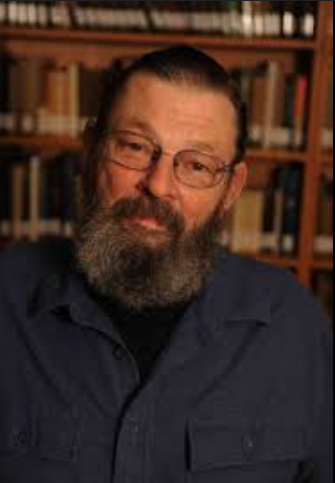
\includegraphics[width=0.6\linewidth]{imagens//secao1/haugeland1985.png}
            \caption{Prof. John Haugeland}
        \end{figure}
    \end{minipage}
    \begin{minipage}{0.5\linewidth}
        \begin{itemize}
        \justifying
            \item \textit{Artificial Intelligence: The Very Idea (1985).}
            \item \aspas{O novo e interessante esforço para fazer os
        computadores pensarem (...) máquinas com mentes, no
        sentido total e literal.}
        \end{itemize}
    \end{minipage}
\end{frame}

% Richard Bellman
\begin{frame}{O que é IA?}
    \begin{minipage}{0.5\linewidth}
        \begin{itemize}
        \justifying
            \item \textit{Artificial Intelligence (1972).}
            \item 
            \aspas{[Automatização de] atividades que associamos ao pensamento humano, atividades como a tomada de decisões, a resolução de problemas, o aprendizado...}
        \end{itemize}
    \end{minipage}
    \begin{minipage}{0.5\linewidth}
        \begin{figure}
            \centering
            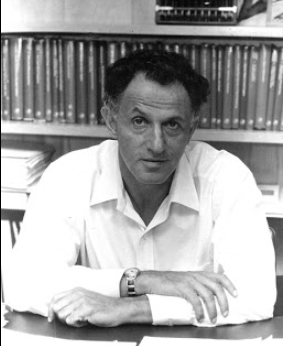
\includegraphics[width=0.6\linewidth]{imagens//secao1/bellman1978.png}
            \caption{Richard Bellman}
            \label{fig:enter-label}
        \end{figure}
    \end{minipage}
\end{frame}

% Raymond Kurzweil
\begin{frame}{O que é IA?}
    \begin{minipage}{0.5\linewidth}
        \begin{figure}
            \centering
            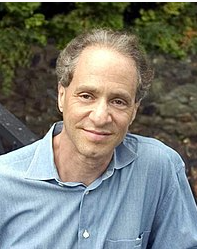
\includegraphics[width=0.5\linewidth]{imagens//secao1/kurzweil.png}
            \caption{Raymond Kurzweil}
        \end{figure}
    \end{minipage}
    \begin{minipage}{0.5\linewidth}
        \begin{itemize}
        \justifying
            \item \textit{The Age of Intelligent Machines (1990).}
            \item 
            \aspas{A arte de criar máquinas que executam funções que exigem inteligência quando executadas por pessoas.”}
        \end{itemize}
    \end{minipage}
\end{frame}

\begin{frame}{O que é IA? }
    \begin{itemize}
        \item 
        \aspas{
        O estudo das faculdades mentais pelo uso de modelos computacionais.
        }
        (Charniak e McDermott, 1985) 
        
        \item 
        \aspas{
        O estudo das computações que tornam possívelperceber, raciocinar e agir.
        }
        (Winston, 1992)
        
        \item 
        \aspas{
        O estudo de como os computadores podem fazer tarefas que hoje são melhor desempenhadas pelas pessoas.
        }
        (Rich and Knight, 1991)
        
        \item 
        \aspas{
        “Inteligência Computacional é o estudo do projeto de agentes inteligentes.
        }
        (Poole et al., 1998) 

        \item 
        \aspas{
        AI... está relacionada a um desempenho inteligente de artefatos.
        }
        (Nilsson, 1998)
    \end{itemize}
\end{frame}
\section{Seção I}
\begin{frame}{Explicações}
    % itemize
    Este é um template que pode ser utilizado para \nocite{Template_Beamer_UFC}:
    \begin{itemize}
        \item Apresentação de Trabalhos Acadêmicos
        \item Apresentação de Disciplinas
        \item Apresentações de Teses e Dissertações
    \end{itemize}

    \vspace{0.4cm} % vertical space
    
    % enumeration
    Para utilizar este template corretamente é importante que:
    \begin{enumerate}
        \item Tenha conhecimento mínimo sobre LaTeX
        \item Ler os comentários no template (explicações)
        \item Ler o README.md (documentação)
    \end{enumerate}

    \vspace{0.2cm}

    \example{Este é um texto de exemplo!} \emph{Texto de Ênfase!}
\end{frame}

%% ---------------------------------------------------------------------------
\subsection{Subseção I}
\begin{frame}{Criando Blocos}
    % Blocks styles
    \begin{block}{Bloco Padrão}
        Texto do corpo do bloco.
    \end{block}

    \begin{alertblock}{Bloco de Alerta}
        Texto do corpo do bloco.
    \end{alertblock}

    \begin{exampleblock}{Bloco de Exemplo}
        Texto do corpo do bloco.
    \end{exampleblock}   
\end{frame}

%% ---------------------------------------------------------------------------
\subsection{Subseção II}
\begin{frame}{Criando Caixas}
    \successbox{testando o success box}

    \pause

    \alertbox{testando o alert box}

    \pause

    \simplebox{testando o simple box}
\end{frame}

%% ---------------------------------------------------------------------------
\subsection{Subseção III}
\begin{frame}{Criando Algoritmos (Pseudocódigo)}
    \begin{algorithm}[H]
        \SetAlgoLined
        \LinesNumbered
        \SetKwInOut{Input}{input}
        \SetKwInOut{Output}{output}
        \Input{x: float, y: float}
        \Output{r: float}
        \While{True}{
          r = x + y\;
          \eIf{r >= 30}{
           ``O valor de $r$ é maior ou iqual a 10.''\;
           break\;
           }{
           ``O valor de $r$ = '', r\;
          }
         } 
         \caption{Algorithm Example}
    \end{algorithm}
\end{frame}

%% ---------------------------------------------------------------------------

\begin{frame}{Inserindo Algoritmos}
    \lstset{language=Python}
    \lstinputlisting[language=Python]{code/main.py}
\end{frame}

%% ---------------------------------------------------------------------------
\begin{frame}{Inserindo Algoritmos}
    \lstinputlisting[language=C]{code/source.c}
\end{frame}

%% ---------------------------------------------------------------------------
\begin{frame}{Inserindo Algoritmos}
    \lstinputlisting[language=Java]{code/helloworld.java}
\end{frame}

%% ---------------------------------------------------------------------------
\begin{frame}{Inserindo Algoritmos}
    \lstinputlisting[language=HTML]{code/index.html}
\end{frame}

%% ---------------------------------------------------------------------------
% This frame show an example to insert multicolumns
\section{Multicolunas}
\begin{frame}{Seção II - Multicolunas}
    \begin{columns}{}
        \begin{column}{0.5\textwidth}
            \justify
            É possível colocar mais de uma coluna utilizando os comandos de $\backslash$begin\{column\}\{\} e $\backslash$end\{column\}
        \end{column}
        \begin{column}{0.5\textwidth}
            \justify
            Porém, o espaçamento deve ser proporcional entre as colunas para que estas colunas não entrem em coflito. O espaçamento é dado pelo segundo argumento do $\backslash$begin.
        \end{column}
    \end{columns}    
\end{frame}

%% ---------------------------------------------------------------------------
% This frame show an example to insert figures
\section{Imagens}
\begin{frame}{Seção III - Figures}
    \begin{figure}
        \centering
        \caption{Emblema da UFC.}
        
\includegraphics[scale=0.3]{libs/emblemufc.pdf}
        \source{Obtido pelo site oficial da UFC \cite{siteufc} \cite{einstein}}
        \label{fig:ufc_emblem}
    \end{figure}
\end{frame}

%% ---------------------------------------------------------------------------
% Reference frames
\begin{frame}[allowframebreaks]
    \frametitle{Referências}
    \printbibliography
\end{frame}

%% ---------------------------------------------------------------------------
% Final frame
\begin{frame}{}
    \centering
    \huge{\textbf{\example{Obrigado!!!}}}
    
    \vspace{1cm}
    
    \Large{\textbf{Contato:}}
    \newline
    \vspace*{0.5cm}
    \large{\email{cicero.hitzschky@alu.ufc.br}}
\end{frame}

\end{document}